\documentclass[border=4pt]{standalone}
\usepackage{tikz}

\begin{document}
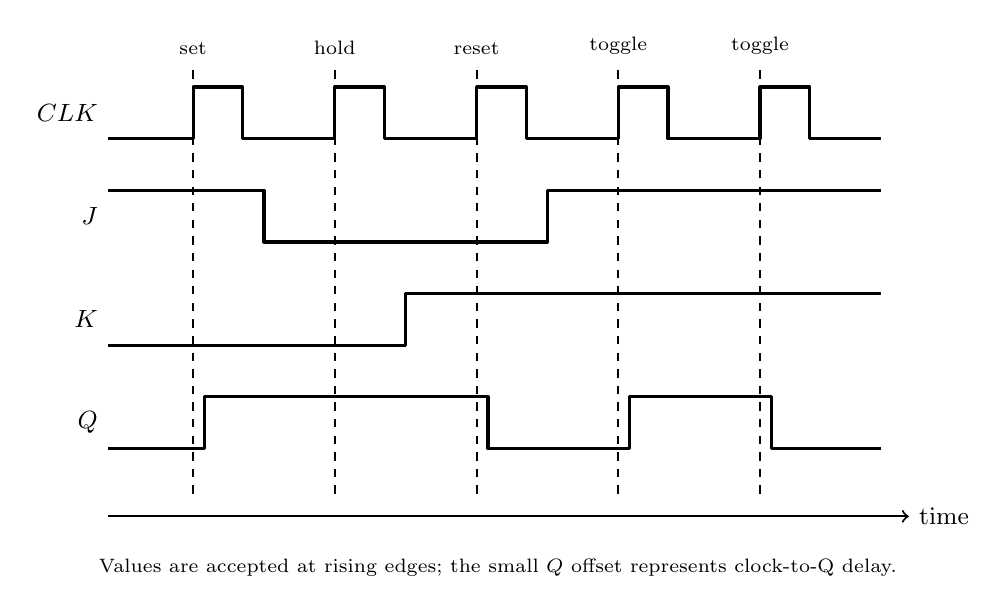
\begin{tikzpicture}[x=0.9cm,y=0.82cm,font=\small,line width=0.75pt,
  thick/.style={line width=1.15pt,line join=round}]
  \draw[->] (0.8,0.15) -- (12.1,0.15) node[right] {time};
  \foreach \y/\name in {6.4/$CLK$,4.8/$J$,3.2/$K$,1.6/$Q$}
    \node[left] at (0.8,\y) {\name};

  \draw[thick] (0.8,6.0) -- (2,6.0) -- (2,6.8) -- (2.7,6.8)
    -- (2.7,6.0) -- (4,6.0) -- (4,6.8) -- (4.7,6.8)
    -- (4.7,6.0) -- (6,6.0) -- (6,6.8) -- (6.7,6.8)
    -- (6.7,6.0) -- (8,6.0) -- (8,6.8) -- (8.7,6.8)
    -- (8.7,6.0) -- (10,6.0) -- (10,6.8) -- (10.7,6.8)
    -- (10.7,6.0) -- (11.7,6.0);
  \draw[thick] (0.8,5.2) -- (3.0,5.2) -- (3.0,4.4)
    -- (7.0,4.4) -- (7.0,5.2) -- (11.7,5.2);
  \draw[thick] (0.8,2.8) -- (5.0,2.8) -- (5.0,3.6) -- (11.7,3.6);
  \draw[thick] (0.8,1.2) -- (2.16,1.2) -- (2.16,2.0)
    -- (6.16,2.0) -- (6.16,1.2) -- (8.16,1.2)
    -- (8.16,2.0) -- (10.16,2.0) -- (10.16,1.2) -- (11.7,1.2);

  \foreach \x/\op in {2/set,4/hold,6/reset,8/toggle,10/toggle} {
    \draw[dashed] (\x,0.5) -- (\x,7.15);
    \node[above,align=center,font=\scriptsize] at (\x,7.15) {\op};
  }
  \node[align=center,font=\scriptsize] at (6.3,-0.65)
    {Values are accepted at rising edges; the small $Q$ offset represents clock-to-Q delay.};
\end{tikzpicture}
\end{document}
